\documentclass{article}
\usepackage{ctex,soul,float,listings,enumerate,hyperref,url,amsfonts,amsmath,graphicx,multirow}
\usepackage{xcolor,tocloft,theorem,numerica,amsmath,mathrsfs}
\usepackage{changes}
\usepackage{fancyhdr}
%%%%%%%%%%%%%%%%%%%%%%%%
\definecolor{AnatationColor}{RGB}{0,139,0}
\lstset{
    backgroundcolor = \color{white},    % 背景色:白色
    basicstyle = \small\ttfamily,           % 基本样式 + 小号字体
    rulesepcolor= \color{white},             % 代码块边框颜色,白色
    breaklines = true,                  % 代码过长则换行
    numbers = left,                     % 行号在左侧显示
    numberstyle = \small,               % 行号字体
    keywordstyle = \color{blue},            % 关键字颜色
    commentstyle =\color{AnatationColor},        % 注释颜色
    stringstyle = \color{red!100},          % 字符串颜色
    frame = shadowbox,                  % 用(带影子效果)方框框住代码块
    showspaces = false,                 % 不显示空格
    columns = fixed,                    % 字间距固定
    %escapeinside={<@}{@>}              % 特殊自定分隔符:<@可以自己加颜色@>
    morekeywords = {as},                % 自加新的关键字(必须前后都是空格)
    deletendkeywords = {compile}        % 删除内定关键字;删除错误标记的关键字用deletekeywords删!
}
\hypersetup{
    colorlinks=true,
    linkcolor=red,
    filecolor=blue,      
    urlcolor=blue,
    citecolor=cyan,
}
\newtheorem{definition}{定义}
\graphicspath{{./Image/}}
%%%%%%%%%%%%%%%%%%%%%%%%
\author{ZeitHaum}
\date{\today}
\title{C++再温习}
\pagestyle{fancy}
%%%%%%%%%%%%%%%%%%%%%%%%
\begin{document}
    \pagenumbering{Roman}
    \maketitle
    \newpage 
    \tableofcontents
    \newpage
    \setcounter{page}{1}
    \pagenumbering{arabic}
    \emph{工欲善其事,必先利其器。}
    \section{语法基础}
    \subsection{include}
    将文件的内容复制到该处,include引入的文件也称为头文件。
    \textbf{增加include的内容只会增加编译时间,对运行时间几乎没有影响。}
    \subsection{main}
    供系统或外部程序调用,return 0 表示运行成功,main函数默认返回return 0。
    \subsection{标识符}
    作为变量名的一组字符,具备以下特征:

    \begin{enumerate}
        \item 允许出现英文、数字、下划线。
        \item 数字不能出现在第一个字符。
        \item 不允许和C++关键词同名。C++关键字可见于:\href{https://www.runoob.com/w3cnote/cpp-keyword-intro.html}{C++ 的关键字(保留字)完整介绍}
    \end{enumerate}
    \subsection{语句}
    需要执行的操作。

    \subsection{终止符}
    C++中即``;'',其是语句的组成部分。

    \subsection{头文件名}
    \begin{figure}[H]
        \centering
        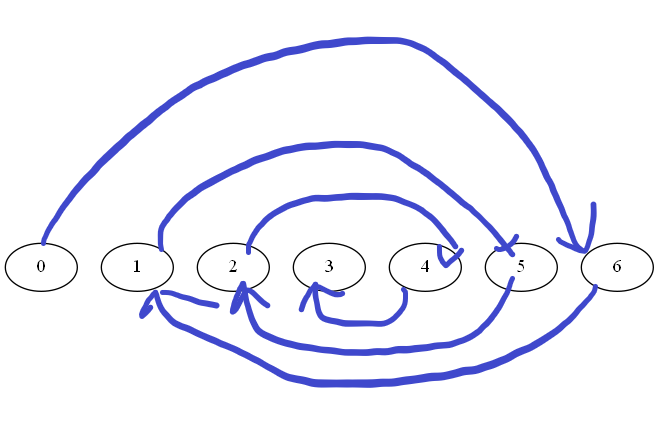
\includegraphics[width = 0.9\textwidth]{fig1.png}
    \end{figure}

    \subsection{名称空间}
    避免重名。使用编译指令语句using 导入。具备两种格式:
    \begin{enumerate}
        \item using namespace std;(全局)
        \item using std::cin;(局部)
    \end{enumerate}

    \subsection{define}
    也称为宏定义语句,本质是文本替换。可以识别变量。例如:
    \begin{lstlisting}[language=c++]
#define pi 3.14159
#define sum(x,y) (x)+(y)
    \end{lstlisting}
    注意由于是文本替换,有可能引起运算顺序上的错误。
    如2*sum(1,2)使用上述文本替换后会错误地先计算乘法。

    define可以递归调用,如:
    \begin{lstlisting}[language=c++]
#define pi 3.1415926
#define calc_circle_area(x) pi*(x)*(x)
    \end{lstlisting}
    

    define可以通过\#函数将标识符转化为字符串,或者通过\#\#将两个标识符合并为新标识符。如:
\begin{lstlisting}[language=c++]
#define tostring(a) (#a)
#define mergestring(a,b) (a##b) 
\end{lstlisting}
    调用第一个宏可以得到值为a的字面量,调用第二个宏可以得到标识符为ab的变量(需要提前定义,否则会报错。)

    可以使用\#undef结束宏定义,在\#undef后的代码将无法使用对应的宏。
    \begin{lstlisting}[language=c++]
#undef pi 
    \end{lstlisting}  

    define的另一大应用是条件编译。首先定义一个没有值的变量,如
    \begin{lstlisting}
#define DEBUG
    \end{lstlisting}
    在代码中可以通过\#if defined(DEBUG)或\#ifdef DEBUG 语句对代码进行选择执行。其对应的取反操作为
    \#if !define(DEBUG) 和\#ifndef DEBUG 。表示其余情况用\#else,结束语句是\#endif。

    \subsection{测试代码}
    对本部分内容的测试代码:

    \lstinputlisting[language=c++]{testSec1.cpp}

    \section{输入输出}

    \subsection{性能}

    std::cin 和std:: cout 相较于C语言的scanf和printf速度较慢。

    使得std::cin速度较慢的原因之一为兼容stdio的开关,可使用std::ios::sync\_with\_stdio(false);关闭。
    此时C++的输入输出和C语言输入输出解除绑定,此时不能同时使用cin和scanf或同时使用cout和printf。

    其次可以解除输入流和输出流的绑定。此时如果需要先cout再cin需要手动flush。如
    \begin{lstlisting}[language=c++]
cin.tie(0);
cout<<"Hello,C++!";
int s;
cin>>s;        
    \end{lstlisting}
    此时执行上述代码就可能会先输入s再输出字符串。注意:\textcolor{red}{endl}会强制清空缓存,因此下述代码不会出现问题: 
    \begin{lstlisting}[language=c++]
cin.tie(0);
cout<<"Hello,C++!"<<endl;
int t;
cin>>t;
    \end{lstlisting}

    其余更多优化(getchar、putchar、fread、fwrite、mmap)等参见\href{https://oi-wiki.org/contest/io/}{OI-wiki-OI优化}.

    \subsection{占位符}
    如下表(\textcolor{red}{注意:C++没有\%b输出二进制的方式。}):

    \begin{table}[H]
        \centering
        \begin{tabular}{cccc}
            \hline
            符号 & 含义 & 符号 & 含义  \\ \hline
            \%d & 十进制整数  & \%g & 小数或者科学计数   \\
            \%f & 浮点数 & \%i & 十进制、八进制、十六进制数   \\
            \%s & 字符串 & \%o & 八进制数 \\
            \%c & 字符 & \%x & 十六进制数  \\
            \%p & 指针 & \%\%  & \%  \\
            \%e & 科学计数法 & \%u  & 无符号数 \\ 
            \%[] & 正则表达式读取字符集  & \%n & 当前已有的字符数 \\\hline
        \end{tabular}
    \end{table}

    \%n的用法举例如下:
    \begin{lstlisting}[language=c++]
int n;
scanf("%s%n",&str,&n);
cout<<tostring(str)<<":"<<str<<" "<<tostring(n)<<":"<<n<<"\n";
    \end{lstlisting}
    在控制台输入``hello,world",终端输出:
    \begin{figure}[H]
        \centering
        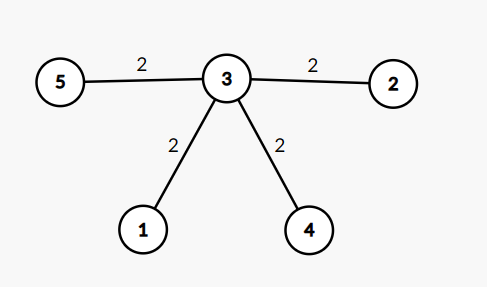
\includegraphics[width = 0.5\textwidth]{fig2.png}
    \end{figure}

    \%[]是C语言的正则表达式用法,当遇到第一个不满足[]内正则表达式的字符便会停止读取。注意需要导入stdio包(不能同时导入iostream包)。
    一个简单的筛选数字的例子如下:

    \begin{lstlisting}[language=c++]
char x[80];
scanf("%[0-9]",x);
printf("%s",x);//注意:x已经是指针,不能再次取地址。
    \end{lstlisting}

    输入``123456789test'',其输出只会读取前几个数字:
    \begin{figure}[H]
        \centering
        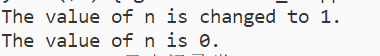
\includegraphics[width = 0.4\textwidth]{fig3.png}
    \end{figure}
    
    \subsection{测试代码}
    \lstinputlisting[language=c++]{testSec2.cpp}

    \section{变量}
    \subsection{内存空间}
        不同类型的变量占据的内存空间不同。
        几个常见的2的幂次:
        \begin{enumerate}
            \item $2^{15} = 32768$
            \item $2^{16} = 65536$
            \item $2^{31} = 2147483648$
            \item $2^{63} \approx 9.2\times 10^18$
        \end{enumerate}
    
        使用sizeof可以查看某个变量所占据的空间(单位字节),库climits可以查看各种类型可以表达的最大值和最小值。
    \subsection{整数}
    short是short integer的简称,long是long integer的简称。
    C++对不同整数的位数定义如下:
    \begin{figure}[H]
        \centering
        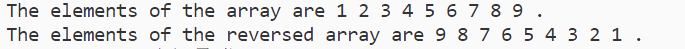
\includegraphics[width = 0.9\textwidth]{fig4.png}
    \end{figure}
    C++默认将证书字面量当作int类型。

    整数类型的省略和顺序调整:
    \begin{figure}[H]
        \centering
        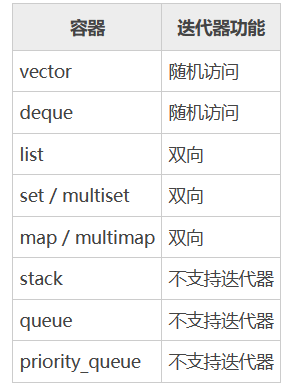
\includegraphics[width = 0.9\textwidth]{fig6.png}
    \end{figure}



    \subsection{bool}
    \textcolor{red}{bool类型占据1字节的空间}。

    \subsection{char}
    占据1字节空间。ASCII码中转义字符的定义如下:
    \begin{figure}[H]
        \centering
        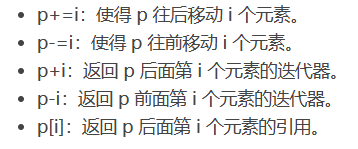
\includegraphics[width = 0.9\textwidth]{fig5.png}
    \end{figure}

    \subsection{void}
    表示无类型。

    \subsection{const}
    表示常量。

    \subsection{浮点数}
    \subsubsection{基本概述}
    C++规定了三种浮点数:float、double、long double。
    在不同的机器中位数一般不一致,通常float 有32位,double 64位,long double 128位。
    可使用cfloat库中的关键字查看。

    \subsubsection{浮点常量}
    浮点常量默认为double类型,如果需要声明为float或long double,需要分别添加后缀F和L(不区分大小写)。

    \subsubsection{浮点数输出}
    这里只介绍一两种通用的方法,更多的方法暂时省略。
    \textbf{1. 保留指定位数}
    使用C语言的格式化输出即可。
    \begin{lstlisting}[language=c++]
float pi = 3.1415926535;
printf("pi = %.6f\n",pi);
    \end{lstlisting}
    \textbf{2. 输出末尾0}
    使用C语言的格式化输出即可,注意C语言不支持long double。
    \begin{lstlisting}[language=c++]
double pi2 = 3.15;
printf("pi = %.6f\n",pi2);
    \end{lstlisting}
    \textbf{3. 舍去多余尾数}
    如果是保留到整数位,可以使用floor函数或者ceil函数,如下例子:
    \begin{lstlisting}[language=c++]
float e = 2.718;
printf("%.0f\n",floor(e));//向下取整,需要引入cmath库
printf("%.0f\n",ceil(e));//向上取整
    \end{lstlisting}
    否则可以先左移再进行取整后再右移。
    \begin{lstlisting}[language=c++]
float test = 29.4525277;
printf("%.2f",floor(test*1e2)/1e2);//保留两位小数(去尾法)
printf("%.2f",floor(test*1e2)/1e2);//保留两位小数(进一法)
    \end{lstlisting}

    \subsection{类型转换}
    \subsubsection{隐式类型转换}
    \textbf{为避免混乱,尽量避免进行隐性类型转换,尤其是无符号和有符号的转换。}
    隐性类型转换的规则(需要特别留意bool和char的转换):
    \begin{figure}[H]
        \centering
        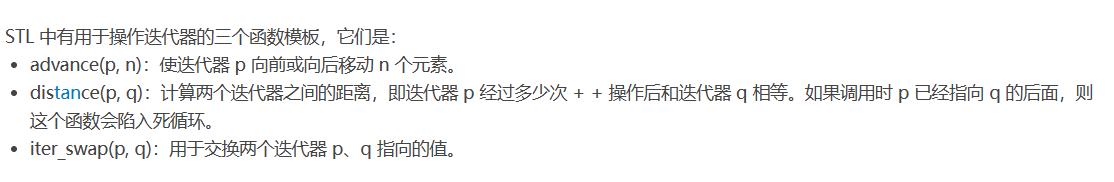
\includegraphics[width = 0.9\textwidth]{fig7.png}
    \end{figure}

    \subsection{强制类型转换}
    有两种方式,如(long)a 和long(a)。
    \textcolor{red}{强制类型转换不会改变原本变量的值,而是创建一个新的变量用于参与表达式运算。}

    \subsection{auto}
    auto是C++ 11加入的特性,用于推测类别。
    注意auto不会进行类型转换,给予字面量时总是和字面量的默认类型一致。
    如0是int,0.0是double。

    \subsection{测试代码}
    \lstinputlisting[language = c++]{testSec3.cpp}

    \section{运算}  
    \subsection{自增自减运算符}
    操作依次从左往右操作。如i++是先返回i再自增。
    尽量避免自增或自减运算符和其他运算符的嵌套,因为C++未明确定义表达式中自增返回值的时机,不同的C++编译器可能返回不同的结果。
    可参考C++ Primerplus中关于顺序点的讨论(P134,第六版)。
    \subsection{逗号运算符}
    起分割运算符的作用,优先级最低,返回最右边的值。
    \textcolor{red}{不建议在普通情况下使用,可能引起误会。}
    \begin{figure}[H]
        \centering
        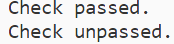
\includegraphics[width = 0.9\textwidth]{fig8.png}
    \end{figure}

    \subsection{赋值语句}
    赋值语句返回值是变量赋值之后的值,一般出现在误将``==''记为``=''的情况下。

    \subsection{运算优先级}
    总体上是!>算术>关系(如大于)>与>或>赋值运算符。
    详细可参见\href{https://baike.baidu.com/item/%E8%BF%90%E7%AE%97%E7%AC%A6%E4%BC%98%E5%85%88%E7%BA%A7/4752611}{百度百科-运算优先级}。

    \subsection{结合性}
    先考虑运算优先级,再考虑结合性。
    结合性分为左结合和右结合,C语言中单目运算符、条件运算符、赋值语句是右结合以外,其他基本均是左结合性。
    可参考帖子\href{https://blog.csdn.net/weixin_41565133/article/details/84332850}{C++运算符结合性(左结合,右结合)}

    \subsubsection{a[i++] 和 a[++i]}
    作为一个例子,背住即可。先计算i++(或者[]内的东西),再计算[]。
    例子:
\begin{lstlisting}[language=c++]
int a[5] = {0,1,2,3,4};
int i = 0;
while(true){
    if(i>=4) break;
    cout<<a[++i]<<endl;
}
int j = 0;
while(true){
    if(j>=4) break;
    cout<<a[j++]<<endl;
}
\end{lstlisting}
    前者输出1、2、3、4后者输出0、1、2、3.

    \subsection{除法的类型转换}
    除法的类型转换完全符合前文中的类型转换。两个整数需要浮点数结果需要先将其中一个数转换为浮点数。

    \subsection{测试代码}
    \lstinputlisting[language=c++]{testSec4.cpp}


    \section{流程控制语句} 
    \subsection{if-else控制语句}
    \subsubsection{if}
        功能介绍略。
        这里介绍一种避免将关系语句误写为赋值语句的方法:
        使用if(3==i)替换if(i==3)。
        \begin{figure}[H]
            \centering
            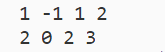
\includegraphics[width = 0.9\textwidth]{fig9.png}
        \end{figure}
    \subsubsection{else}
        略。
    \subsubsection{else if}
        略。

    \subsection{逻辑运算}
    \subsubsection{\&\&、||、!}
    略。
    \subsubsection{细节}
    \textbf{1.}
    使用a>3 \&\& a<5 而不是 3<a<5。后者会被视为(3<a)<5。
    \textbf{2.}
    符号!的优先级高于关系运算符,因此取反要括起来。比如!x>1表示判断!x和1的大小关系。
    \textbf{3.} 
    C++ 支持使用and、or、not替换\&\&、||、!。
    例如:
    \begin{lstlisting}[language=c++]
int x = 3;
int y = 2;
if(3==x and y>1 and y<3)cout<<"If test PASS!"<<endl;
    \end{lstlisting}

    \subsection{cctype字符函数库}
    提供判断字符(char)类型的很多函数,比用if-else更方便。如可以使用isalpha()判断是否为字母。
    以下是一个例子:
    \begin{lstlisting}
string a_str = "Hello,world!";
for(int i = 0;i<a_str.size();i++){
    if(isalpha(a_str[i]))cout<<a_str[i];
}
cout<<endl;
    \end{lstlisting}
    程序的输出结果为Helloworld。
    cctype其他函数如下:
    \begin{figure}[H]
        \centering
        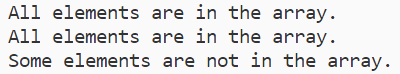
\includegraphics[width = 0.9\textwidth]{fig10.png}
    \end{figure}
    
    \subsection{?:}
    ?:是C++唯一一个三目运算符。
    注意嵌套问题,当判断条件过多时推荐使用if-else语句。

    \subsection{switch-case语句}
    switch处填入一个表达式(值必须在整数集合内),case语句填入一个整数值。
    根据表达式的值,程序跳转到对应的语句\textbf{依次}执行代码。要避免依次执行请使用break语句。
    如以下例子:
    \begin{lstlisting}[language=c++]
int z = 0;
while (1)
{
    if(z>=4)break;
    switch (z)
    {
    case 0:
        cout<<"z is 0."<<endl;
        break;
    case 1:
        cout<<"z is 1."<<endl;
        break;
    case 2:
        cout<<"z is 2."<<endl;
        break;
    default:
        cout<<"Error:z has a wrong value."<<endl;
        break;
    }
    z++;
}
    \end{lstlisting}

    输出结果:
    \begin{figure}[H]
        \centering
        \includegraphics[width = 0.6\textwidth]{fig12.png}
    \end{figure}

    \subsection{break 和 continue}
    略。

    \subsection{测试代码}
    \lstinputlisting[language=c++]{testSec5.cpp}

    \section{循环}
    \subsection{for}
    \subsubsection{基本结构}
    for循环基本结构:
    \begin{figure}[H]
        \centering
        \includegraphics[width = 0.5\textwidth]{fig13.png}
    \end{figure}
    任何一个部分都可以省略(;不能省略),省略判断条件默认为真。

    for循环是入口条件循环,每轮循环开始前都将计算循环条件,因此当循环条件较为复杂时会降低效率(视编译器而定)。

    \subsubsection{和逗号运算符使用的技巧}
    for循环的另一个技巧是和逗号运算符的使用,参见以下反转字符串的方法:
    \begin{lstlisting}[language=c++]
string s = "Hello,C++!";
int i,j;//必须提前声明,int j = s.size()-1不是一个表达式语句。
for(i = 0,j = s.size()-1;i<j;i++,j--){
    char c = s[i];
    s[i] = s[j];
    s[j] = c;
}
cout<<s<<endl;  
    \end{lstlisting}
    输出:
    \begin{figure}[H]
        \centering
        \includegraphics[width = 0.4\textwidth]{fig14.png}
    \end{figure}

    \subsubsection{基于范围的循环}
    C++引入的新特性,类似于Python的范围遍历,\textbf{通常和auto结合使用}。
    一个简单的例子如下,用于输出数组全部元素。
    \begin{lstlisting}[language=c++]
float f[4] = {0.1,0.2,0.3,1.1};
for(auto x:f){
    cout<<x<<endl;
}
    \end{lstlisting}

    \subsection{while}
    功能略。永远循环的两种等价写法:
    \begin{enumerate}
        \item for(;;)
        \item while(1)
    \end{enumerate}

    \subsection{do-while}
    先执行语句再判断条件,一般不常用。

    \subsection{测试代码}
    \lstinputlisting[language = c++]{testSec6.cpp}
    
    \section{C++高级数据类型}
    \subsection{一维数组}
    \subsubsection{基本概述}
    只能存访相同类型,声明长度必须是常量(被const修饰)。
    \subsubsection{数组越界}
    会触发段错误或者修改意外之外的值。
    \subsubsection{数组初始化}
    直接阅读以下代码和注释即可:
    \begin{lstlisting}[language=c++]
//初始化数组
int arr1[4];
int arr2[3] = {1,2,3};
int arr3[7] = {1,2,3};//不满默认补零。
int arr4[10] = {0};//快速初始化一个全为0的数组
int arr5[] = {12,23,445,464,1225};//自动推测数组长度 
    \end{lstlisting}

    打印数组的结果如下,可用于检验数组生成结果:
    \begin{figure}[H]
        \centering
        \includegraphics[width = 0.5\textwidth]{fig15.png}
    \end{figure}
    注意:在程序的非静态区声明的数组取值不一定为默认值(0)。

    \subsubsection{C++11的数组初始化}
    可以省略``=''号,若``\{\}''中无内容将会视为全0.如以下代码:
    \begin{lstlisting}[language=c++]
int arr6[] {1,3,5,7,9};
int arr7[5] {};
    \end{lstlisting}

    \subsection{多维数组}
    多维数组实质上在计算机内仍是按一维数组存储,不过其下标进行了对应的换算。
    数组存储的方法有很多种,如二维数组有按行优先和按列优先两种存储方法。实际中常常尽量选择局部性良好的方法。

    另外,多维数组应尽量使其存储位置连续,这样可以利用Cache加速实现性能提升。
    C++中vector速度慢于自带的多维数组的原因便是vector行间数据存储不连续。详情可见\href{https://blog.csdn.net/qq_42080098/article/details/124357242}{C++多维vector为什么比多维数组慢}。
    
    \subsection{字符串}
    \subsubsection{C风格字符串}
    一个包含`$\backslash$0'的char数组,且`$\backslash$0'视为字符串的结束,该字符以后的字符被忽略。

    \textbf{1.初始化}

    可以使用数组或字符串的形式初始化,注意数组的空间要给够。以下是例子:
    \begin{lstlisting}[language=c++]
//字符串
char str1[15] = {'H','e','l','l','o',',','w','o','r','l','d','!','\0'};//末尾'\0'不可省略。
char str2[15] = "Hello,world!";//多余空间均被赋值为'/0'。
char str3[] = "Hello,world!";//自动推测
    \end{lstlisting}

    \textbf{2.拼接字符串常量}
    
    C++允许以下操作:
    \begin{lstlisting}[language=c++]
cout<<"Hello"
",world!"<<endl;
    \end{lstlisting}
    当字符串很长时此技巧很有用。

    \textbf{3.csring 库}
    
    cstring库(或string.h)提供了一些与C风格相关的函数,如strlen()和strcmp函数。
    \begin{lstlisting}[language=c++]
printf("The size of str1 is %d.\n",strlen(str1));
if(strcmp(str1,str2)) printf("%s","str1 = str2.\n");
else printf("%s","str1!=str2.\n");
    \end{lstlisting}
    注意判断字符串相等不能使用"==",这里"str1==str2"返回的是两者地址是否相同,如下:
    \begin{lstlisting}[language=c++]
printf("The size of str1 is %d.\n",strlen(str1));
if(str1==str2) printf("%s","The address of str1 is equal to str2.\n");
else printf("%s","The address of str1 is not equal to str2.\n");
    \end{lstlisting}

    \subsubsection{C++风格字符串}
    使用的是string库,具体用法参照官方文档。

    \subsubsection{字符串I/O:读取一行}
    对于C风格字符串,有cin.get(str,length)和cin.getline(str,lenth)两个函数。
    这里length表示读取的字符串最大长度。
    当读取到换行符或者读取字符超过最大长度限制将会停止读取。
    对于C++风格字符串,有getline(cin,str)一个函数。
    示例如下:
    \begin{lstlisting}[language=c++][H]
char str5[50];
char str6[50];
char test_c;
string str7;
cout<<"Readline begin."<<endl;
cin.getline(str5,20);
cin.get(str6,20);
//get会保留换行符,因此c必为换行符;对于cin可以忽略。
scanf("%c",&test_c);
cout<<int(test_c)<<endl;
getline(cin,str7);
cout<<"Readline end."<<endl;
    \end{lstlisting}
    输出可见test\_c的ASCII编号为10,正是代表换行符。
    \begin{figure}[H]
        \centering
        \includegraphics[width = 0.5\textwidth]{fig16.png}
    \end{figure}

    \subsubsection{其他形式的字符串}
    如下表:
    \begin{table}[H]
        \centering
        \begin{tabular}{cccccc}
            \hline
             类型名称 & 别称 &  适用版本 & 占用比特数 & 字面量前缀 & 备注 \\ \hline
             wchar\_t & 宽字符类型 & C++ & 16 & L & 用于国际化 \\
             char16\_t & - & C++11 & 16 & u & - \\
             char32\_t & - & C++11 & 32 & U & - \\ 
             \hline
        \end{tabular}
    \end{table}
    另外C++11还可以使用前缀``u8''指定编码格式,``R''表示原始字符类型。

    \subsection{结构体}
    C语言不能省略struct. 

    \subsubsection{结构体初始化}
    如下代码,解析见注释:
    \begin{lstlisting}[language=c++]
//结构体声明
struct test
{
    int x;
    int y;
    double d;
    string s;
};
//采用数组的方式初始化
test t1 = {1,2,1.2,"test"};//不省略等号
test t2 {1,2,1.3,"test2"};//省略等号(C++11)
cout<<t1.d<<endl;
cout<<t2.s<<endl;
//声明结构体的同时初始化变量
struct position
{
    float x;
    float y;
} p1,p2;
cout<< p1.x-p2.x <<endl;

//省略结构体名,以后无法使用结构体名新建变量
struct {
    double x;
    double y;
    string name;
} shop = {1.0,1.0,"Cake"};
cout<<shop.name<<endl;
    \end{lstlisting}

    \subsubsection{结构数组}
    略。
    \subsubsection{结构中的位字段}
    使用``:''指定占据特定位数的结构成员,常用于低级编程。此处不展开。

    \subsection{共用体}
    只能同时存储多种数据类型中的一种,当一个变量拥有多种不同的数据类型时可以使用。
    常用于嵌入式编程节省内存,普通系统不常用,此处不展开。

    \subsection{枚举}
    \subsubsection{声明和赋值}
    一种创建符号常量的方法,声明与struct类似。
    默认将枚举赋值为0,1,2,...,枚举类型能隐式转换为整数,但是整数不可以隐式转换为枚举类型。
    枚举类型只定义了赋值语句,其他操作未定义。当整数超出了枚举类型范围也是未定义行为,在某些编译器中将会报错。
    例子如下:
    \begin{lstlisting}[language = c++]
enum color {red,green,white,black};
color c = red;
cout<<c<<endl;
//color c2 = 3; Error!
color c2 = (color)3;//OK 
    \end{lstlisting}

    \subsubsection{指定枚举的值}
    枚举类型允许有相同的值,枚举有效范围为枚举值中最大的值。
    C++允许枚举被赋值为long long 类型,不允许非整数类型。
    例子如下:
    \begin{lstlisting}[language=c++]
enum bits {a = 2,one = 2,two = 4,three = 8,four = 16,super_long = 2147483649L};//可声明为long long.
bits b = (bits)6;//Valid, In range.
cout<<bits::super_long<<endl;//访问枚举值使用::符号
    \end{lstlisting}

    \subsection{测试代码}
    \lstinputlisting[language=c++]{testSec7.cpp}

    \section*{参考资料}
    \addcontentsline{toc}{section}{参考资料}
    [1]. \href{https://OI-wiki.org}{OI-wiki}.

    [2]. C++ Primerplus中文版(第六版).

    [3]. \href{https://www.runoob.com/note/26809}{菜鸟教程}

    [4]. \href{https://blog.csdn.net/}{CSDN}.
\end{document}
